\documentclass[landscape,a1paper,fontscale=0.5]{poster}

\usepackage{graphicx}  % Required for including images
\graphicspath{{figures/}} % Directory in which figures are stored

\usepackage{amsmath}
\usepackage{amssymb}
\usepackage{bm}

\usepackage[font=small,labelfont=bf]{caption}

\definecolor{light}{HTML}{81C4E6} 
\definecolor{medium}{HTML}{3399CC} 
\definecolor{dark}{HTML}{0070A8} 

\begin{document}

\begin{poster}{
headerborder=closed, % Adds a border around the header of content boxes
colspacing=1em, % Column spacing
bgColorOne=white, % Background color for the gradient on the left side of the poster
bgColorTwo=white, % Background color for the gradient on the right side of the poster
borderColor=light, % Border color
headerColorOne=medium, % Background color for the header in the content boxes (left side)
headerColorTwo=medium, % Background color for the header in the content boxes (right side)
headerFontColor=white, % Text color for the header text in the content boxes
boxColorOne=white, % Background color of the content boxes
textborder=rectangle, % Format of the border around content boxes, can be: none, bars, coils, triangles, rectangle, rounded, roundedsmall, roundedright or faded
eyecatcher=true, % Set to false for ignoring the left logo in the title and move the title left
headerheight=0.1\textheight, % Height of the header
headershape=roundedright, % Specify the rounded corner in the content box headers, can be: rectangle, small-rounded, roundedright, roundedleft or rounded
headerfont=\Large\bf\textsc, % Large, bold and sans serif font in the headers of content boxes
%textfont={\setlength{\parindent}{1.5em}}, % Uncomment for paragraph indentation
linewidth=1pt % Width of the border lines around content boxes
}
%----------------------------------------------------------------------------------------
%	TITLE PARAMETERS
%----------------------------------------------------------------------------------------
{
\includegraphics[height=5em]{mmr-text.png}}
{\bf\textsc{Numerical simulation of dynamic processes in a nuclear reactor \\ \vspace{0.2em} by state change modal method}}
{Alexander Avvakumov$^1$ \quad Valery Strizhov $^2$ \quad Petr Vabishchevich $^{2,3}$ \quad \underline{Aleksandr Vasilev $^{3,a}$} \\
\normalsize{$^1$ National Research Center "Kurchatov Institute", Moscow \quad
$^2$ Nuclear Safety Institute, Russian Academy of Sciences, Moscow \quad
$^3$ North-Eastern Federal University, Yakutsk \quad
$^a$ haska87@gmail.com}}
{
\includegraphics[height=5em]{logoNEFU.png}}

%----------------------------------------------------------------------------------------
%	INTRODUCTION
%----------------------------------------------------------------------------------------
\headerbox{Introduction}{name=introduction,column=0,row=0}{
%\hspace{1em} In practical calculations of nuclear reactors, as a rule,  simpler systems of equations in the multigroup diffusion  approximation  are used [1].

\hspace{1em} Quasistatic method [1]. 
One of which depends on the time and is related to the amplitude, the second (shape function) describes the spatial distribution. The shape function is often associated with the fundamental eigenfunction of certain eigenvalue problems for neutron diffusion equations. 

\hspace{1em} Modal method [2].
In this case, the solution is represented in the form of a sum of several dominant eigenvalues with time-dependent coefficients.

\hspace{1em} Nonstationary processes can naturally be described on the basis of the approximate solution expansion in time-eigenvalue of  $\alpha$-eigenvalue problem [3].
We deal with an unbound system of equations for the coefficients. It should also be noted that the eigenvalues are complex for both $\lambda$- and 
$\alpha$-eigenvalue problem. To set the initial state, this leads to the need to solve the appropriate adjoint spectral problems.

\hspace{1em} In this paper, we formulate a general strategy for the approximate solution of nonstationary problems of neutron transport in nuclear reactors, which is oriented to fast real-time calculations using the SCM method.

\vspace{0.5em}
[1] Dodds~Jr, H.~L. //Nuclear Science and Engineering. --- 1976. --- Vol. 59~(3). --- P. 271--276.

[2] Stacey, W.~M. //The MIT Press. ---  1967. 

[3] Avvakumov, A.~V. et al. //Annals of Nuclear Energy. --- 2017. --- Vol. 99. --- P. 68--79. 

}

%----------------------------------------------------------------------------------------
%	Problem statement
%----------------------------------------------------------------------------------------
\headerbox{Problem statement}{name=statement,column=0,below=introduction,above=bottom}{
Define vectors $\bm \phi = \{\phi_1, \phi_2, ..., \phi_G\}$, $\bm c = \{c_1, c_2, ..., c_M\}$ and matrix: 
\[
\begin{split}
	 V &= (v_{g g'}), \quad\phantom{12345} v_{g g'} = \delta_{g g'} v_g^{-1}, \\
	 D &= (d_{g g'}), \quad\phantom{12345} d_{g g'} = - \delta_{g g'} \nabla \cdot D_g \nabla, \\
	 S &= (s_{g g'}), \quad\phantom{12345} s_{g g'} =  \delta_{g g'} \Sigma_{rg} - \Sigma_{s,g'\rightarrow g}, \\ 
	 R &= (r_{g g'}),	\quad\phantom{12345} r_{g g'} = (1-\beta)\chi_g \nu \Sigma_{fg'}, \\
	 B &= (b_{g m}), \quad\,\,\phantom{1234} b_{g m} = \widetilde{\chi}_g \lambda_m, \\
	\Lambda &= (\lambda_{m m'}), \quad\phantom{12} \lambda_{m m'} = \lambda_m \delta_{m m'}, \\
	Q &= (q_{mg}), \quad\,\,\phantom{1234} q_{mg} = \beta_m \nu \Sigma_{fg}, \\
	g, g' &= 1,2, ..., G, \quad m, m' = 1,2, ....,M. 
\end{split}
\]
%\[
%	V = (v_{g g'}), 
%	\,
%	v_{g g'} = \delta_{g g'} v_g^{-1}, 
%	\quad
%	D = (d_{g g'}), 
%	\,
%	d_{g g'} = - \delta_{g g'} \nabla \cdot D_g \nabla,
%\]
%\[
%	S = (s_{g g'}), 
%	\,
%	s_{g g'} =  \delta_{g g'} \Sigma_{rg} - \Sigma_{s,g'\rightarrow g}, 
%	\quad
%\]
%\[
%	R = (r_{g g'}),	 r_{g g'} = (1-\beta)\chi_g \nu \Sigma_{fg'},
%	\quad
%	B = (b_{g m}), 
%	\, 
%	b_{g m} = \widetilde{\chi}_g \lambda_m, 
%\]
%\[
%	\Lambda = (\lambda_{m m'}), \,  \lambda_{m m'} = \lambda_m \delta_{m m'},
%	\quad
%	Q = (q_{mg}), \,  q_{mg} = \beta_m \nu \Sigma_{fg},
%\]
%\[ 
%	g, g' = 1,2, ..., G, \quad m, m' = 1,2, ....,M. 
%\]
Multigroup diffusion equation:
\begin{eqnarray*}
V \frac{d \bm \phi}{d t} + (D+S) \bm \phi = R \bm \phi + B\bm c,
\\
\frac{d \bm c}{d t} + \Lambda \bm c = Q \bm \phi. 
\end{eqnarray*}  
Here $\phi_g(\bm x,t)$ is the neutron flux,
$v_g$ is the effective neutron velocity,
$D_g(\bm x)$ -- diffusion coefficient, 
$\Sigma_g(\bm x,t)$ -- removal cross-section,
$\Sigma_{s,g'\rightarrow g}(\bm x,t)$ -- scattering cross-section,
$\nu\Sigma_{fg}(\bm x,t)$ -- generation cross-section, 
$\chi_g$ ($\widetilde\chi_g$) -- fraction of neutrons, 
$c_m$ -- delayed neutron source density,  $\lambda_m$ -- decay constant of the delayed neutron sources.

The Cauchy problem is solved under the initial conditions:
\begin{eqnarray*}
\bm \phi(0) = \bm \phi^0, \quad  \bm c(0) = \bm c^0,
\end{eqnarray*}  
where $\bm \phi^0 = \{ \phi_1^0,  \phi_2^0, ...,  \phi_G^0 \}, \quad
\bm c^0 = \{ c_1^0,  c_2^0, ...,  c_M^0 \}$.
}

\headerbox{State change cheme}{name=approximation,column=1,row=0}{
The state of the reactor is characterized by the constant coefficients of the system of multigroup diffusion equations.
\begin{center}
    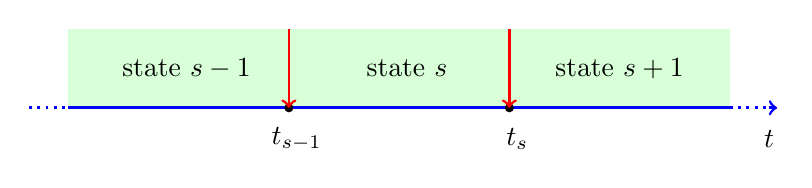
\begin{tikzpicture}
      \filldraw [color=green!15] (-0.5,0) rectangle +(8.4,1);
      \draw [dotted, line width=1, color=blue] (-1,0) -- (-0.5,0);
      \draw [line width=1, color=blue] (-0.5,0) -- (7.9,0);
      \draw [dotted, line width=1, color=blue] (7.9,0) -- (8.4,0);
      \draw [->, line width=1, color=blue] (8.4,0) -- (8.5, 0);
      \filldraw [black] (2.3,0) circle (0.05);
      \filldraw [black] (5.1,0) circle (0.05);
      \draw  (1.0,0.5) node {state $s-1$};  
      \draw  (3.8,0.5) node {state $s$};  
      \draw  (6.5,0.5) node {state $s+1$};  
      \draw  (2.4,-0.4) node {$t_{s-1}$}; 
      \draw  (5.2,-0.4) node {$t_{s}$}; 
      \draw  (8.4,-0.4) node {$t$}; 
      \draw [->, line width=1, color=red] (2.3,1) -- (2.3,0);
      \draw [->, line width=1, color=red] (5.1,1) -- (5.1,0);
    \end{tikzpicture}
\end{center}

Dynamic processes in a nuclear reactor can be considered as a change of states. 
At a certain time $t = t_s, \ s = 1,2, ...$ an instantaneous change of state occurs. 
The state $s$ is defined by the parameters in equations:
\[
 V(t) = V(t_s), \quad  D(t) = D(t_s), \quad  S(t) = S(t_s), \quad  R(t) = R(t_s),
\] 
\[
 B(t) = B(t_s), \quad \Lambda(t) = \Lambda(t_s), \quad  Q(t) = Q(t_s)\\
\]
\[
t_{s-1} < t \leq t_s, \quad s = 1,2, ... 
\] 

}

%----------------------------------------------------------------------------------------
%	Componentwise splitting schemes
%----------------------------------------------------------------------------------------
\headerbox{Modal approximation}{name=componentwise,column=1,below=approximation,above=bottom}{
Non-stationary process at a separate stage is based on modal approximation.
Let's $\bm u = \{\bm \phi, \bm c\}, \ \bm \phi(t_{s-1}) = \bm \phi^s, \ \bm c(t_{s-1}) = \bm c^s$.
In a separate stage s the following system is considered
\begin{eqnarray*}
 \bm B \frac{d \bm u}{d t} + \bm A \bm u = 0,
 \quad t_{s-1} < t \leq t_s,
\end{eqnarray*}
with constants
\[
 \bm A = 
 \begin{pmatrix}
 D(t_s)+S(t_s) - R(t_s) &  - B(t_s) \\
 - Q(t_s) & \Lambda(t_s) 
 \end{pmatrix} ,
 \quad  \bm B = 
 \begin{pmatrix}
 V(t_s) & 0 \\
 0 & I 
 \end{pmatrix}.
\] 
Supplemented by the corresponding initial condition
\begin{eqnarray*}
 \bm u(t_{s-1}) = \bm u^s .
\end{eqnarray*}
The matrices $\bm A_h$ and $\bm B_h$ are real and asymmetric.

The modal approximation corresponds to the representation of the approximate solution  ($\bm u_h \approx \bm u_N$) of problem  in the following
\[
 \bm u_N(\bm x, t) =
 \sum_{n=1}^{N} a_n(t) \bm w_n(\bm x),
\]
where $N$ is the number of dominant eigenvalues of the spectral problem, 
$\bm w_n(\bm x)$ --- corresponding eigenfunctions.

We consider $\alpha$-eigenvalue problem
\[
 \bm A_h \bm v = \lambda  \bm B_h \bm v .
\]
Then we obtain
\[
\begin{split}
 a_n(t) \bm w_n(\bm x) & = b_n \mathrm{Re} \big ( \exp(-\lambda_n (t-t_{s-1})) \bm v_n(\bm x) \big ), \\
 a_{n+1}(t) \bm w_{n+1}(\bm x) & = b_{n+1} \mathrm{Im} \big ( \exp(-\lambda_n (t-t_{s-1})) \bm v_n(\bm x) \big ) .
\end{split}
\] 
A special attention should be paid to define the coefficients $a_n(t_{s-1}) = b_n, \ n = 1,2, ..., N$.
For this, the initial condition is involved. For example, in the case of real eigenvalues, we have
\vspace{-0.5em}
\[
 \bm u_h^s (\bm x) = \sum_{n=1}^{N_h} b_n \bm v_n(\bm x) .
\]  
}

%----------------------------------------------------------------------------------------
%	Convection-diffusion problem
%----------------------------------------------------------------------------------------

\headerbox{Adjoint spectral problem}{name=problem,column=2,aligned=componentwise,above=bottom}{
Consider the adjoint spectral problem 
\[
 \bm A_h^T \widetilde{\bm v}  = \lambda  \bm B_h^T \widetilde{\bm v} .
\]
The eigenfunctions of problems  are orthogonal  in the sense of the equality
\[
  (\bm B_h \bm v_n, \widetilde{\bm v}_m)= 0, 
  \quad m \neq n,
  \quad m, n = 1,2, ..., N_h.
\] 
In view of this, one can obtain
\[
 b_n = \frac{1}{(\bm B_h \bm v_n, \widetilde{\bm v}_n)} (\bm u_h^s, \bm B_h \widetilde{\bm v}_n),
 \quad n = 1,2, ..., N_h .  
\]
In the approximate solution of problem  only the first $N$ coefficients  $b_n$ are used:
\[
 \bm c_h^s (\bm x) \approx  \sum_{n=1}^{N} b_n \bm c_n(\bm x) ,
\]
where $\bm v_n (\bm x) = (\bm \phi_n (\bm x), \bm c_n (\bm x))$.
In this case, the spectral problems are solved for $N$ dominant eigenvalues.

\begin{description}
\item[Off-line calculation.] 
Calculation of the coefficients of the mathematical model of the multigroup diffusion approximation for the isolated reactor states, which is performed in advance. 
The status passport also includes calculated dominant eigenvalues and eigenfunctions of the  $\alpha$-eigenvalue problem. 
These data can be supplemented by dominant eigenvalues and eigenvalues of the conjugate eigenvalue problem.
\item[On-line calculation.]
Real-time modeling is carried out on the basis of the modal solution of the problem.
The coefficients in the representation are calculated from the initial condition. 
The solution for other time intervals is determined according to modal approximation.   
\end{description} 
}

%----------------------------------------------------------------------------------------
%	Vector additive schemes
%----------------------------------------------------------------------------------------

\headerbox{Time scale processes}{name=vector,column=2,row=0,above=problem}{
The initial condition includes two components 
\[
\bm u_h^s (\bm x) = (\bm \phi_h^s (\bm x), \bm c_h^s (\bm x)).
\]
Dynamic behaviour of these components is due to different time-scale processes. 
\vspace{1em}

Delayed neutrons source determines \textbf{slow processes}, when  $\bm c(\bm x,t)$ changes slightly with the reactor state change. In contrast, neutron flux $\bm \phi(\bm x,t)$ determines \textbf{fast processes} when the reactor state changes. 

\vspace{1em}
By virtue of this separation of dynamic processes, we model the slow phase of the dynamics of the reactor with modal approximation and orientate ourselves on the approximate prediction of the initial state for delayed neutrons, only the function  $\bm c_h^s (\bm x)$ is approximated. The approximation  $\bm \phi_h^s (\bm x)$ is not of interest to us, we do not model a fast phase of the state change.
}

\headerbox{Numerical experiments}{name=experiments,column=3,aligned=vector,above=bottom}{
The dynamics of the VVER-1000 (Fig 1.) reactor during the transition from the supercritical mode to the subcritical mode

\begin{minipage}{0.5\textwidth}
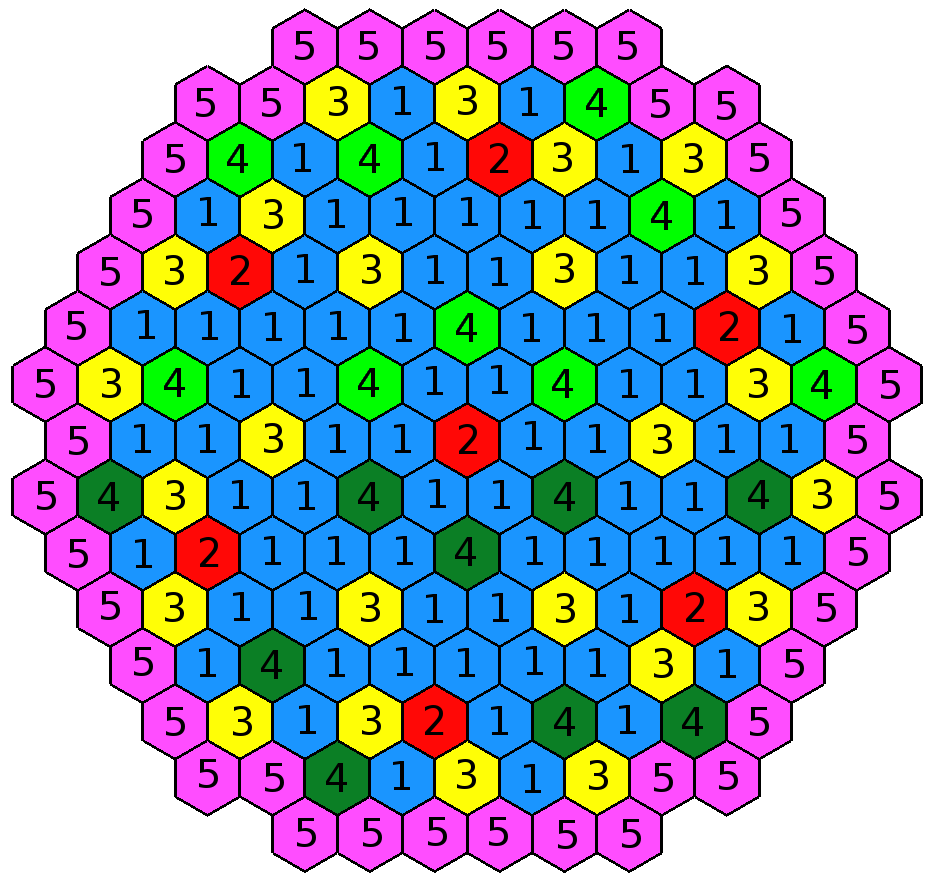
\includegraphics[width=0.9\linewidth]{geo.png}
\begin{center}
\vspace{-1em}
Fig. 1 Geometry
\end{center}
\end{minipage}
\begin{minipage}{0.5\textwidth}
\begin{itemize}
\setlength\itemsep{0em}
\item two-dimensional
\item two group instantaneous and one group of delayed neutrons
\item triangles per cassette $\kappa$ \\ varies from 6 to 96
\item order of finite elements $p$ varies from 1 to 3
\item two types of perturbation
\end{itemize}
\end{minipage}

\vspace{0.5em}
The coefficients $b_n, \ n = 1,2, ..., N$, $N=50$ of the approximate solution with the initial condition are shown in Fig. 2.

\begin{minipage}{0.5\textwidth}
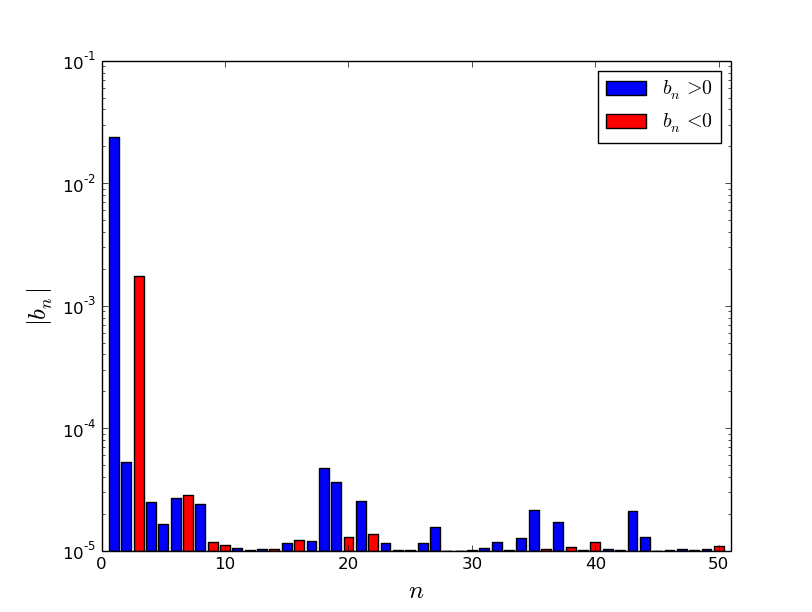
\includegraphics[width=1\linewidth]{12.png}  
\begin{center}
\vspace{-1em}
Fig 2. Approximate solution coefficients
\end{center}
\end{minipage}
\begin{minipage}{0.5\textwidth}
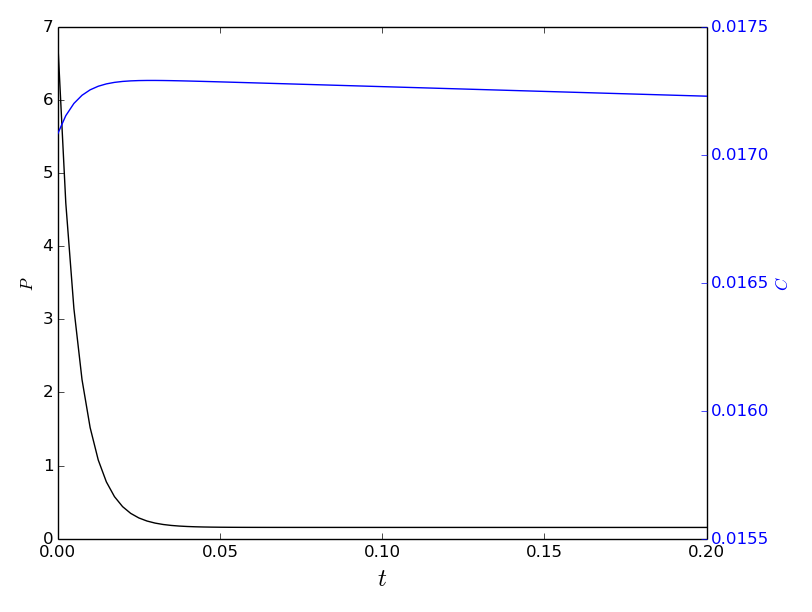
\includegraphics[width=1\linewidth] {14.png}
\begin{center}
\vspace{-1em}
Fig 3. Neutronic power
\end{center}
\end{minipage}

\vspace{0.5em}
The dynamics of the neutron power of the nuclear reactor  $P(t) = \int_{\Omega} (\nu\Sigma_{f1} \phi_1(\bm x,t) + \nu\Sigma_{f2} \phi_2(\bm x,t))  d \bm x$ and the delayed neutrons source $C(t) = \int_{\Omega} c(\bm x,t) d \bm x$ at the initial stage during the transition from the critical state to the subcritical is shown in Fig. 3. 

\vspace{0.5em}
The beginning and the end of the fast phase are illustrated through the
calculational data shown in Fig. 4.

\begin{center}
\begin{minipage}{0.051\linewidth}
\center{1} \\
\end{minipage}
\hfill
\begin{minipage}{0.3\linewidth}
\center{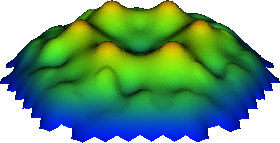
\includegraphics[width=1\linewidth]{13-11.png}} \\
\end{minipage}
\hfill
\begin{minipage}{0.3\linewidth}
\center{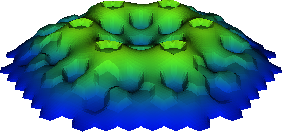
\includegraphics[width=1\linewidth]{13-12.png}} \\
\end{minipage}
\hfill
\begin{minipage}{0.3\linewidth}
\center{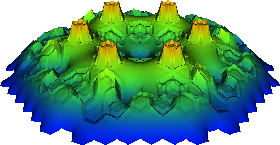
\includegraphics[width=1\linewidth]{13-13.png}} \\
\end{minipage}

\begin{minipage}{0.051\linewidth}
\center{2} \\
\end{minipage}
\hfill
\begin{minipage}{0.3\linewidth}
\center{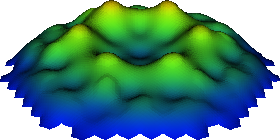
\includegraphics[width=1\linewidth]{13-21.png}} \\
\end{minipage}
\hfill
\begin{minipage}{0.3\linewidth}
\center{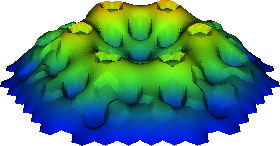
\includegraphics[width=1\linewidth]{13-22.png}} \\
\end{minipage}
\hfill
\begin{minipage}{0.3\linewidth}
\center{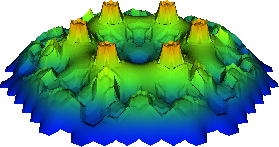
\includegraphics[width=1\linewidth]{13-23.png}} \\
\end{minipage}

\begin{minipage}{0.051\linewidth}
\center{~} \\
\end{minipage}
\hfill
\begin{minipage}{0.3\linewidth}
\center{a} \\
\end{minipage}
\hfill
\begin{minipage}{0.3\linewidth}
\center{b} \\
\end{minipage}
\hfill
\begin{minipage}{0.3\linewidth}
\center{c} \\
\end{minipage}
\hfill
Fig 4. Function $\bm u(\bm x, 0)$ (string 1) and function  $\bm u_N(\bm x, 0)$ (string 2): a --- neutron flux of group 1, b --- neutron flux of group 2, c --- delayed neutrons source.
\end{center}

\begin{minipage}{0.5\textwidth}
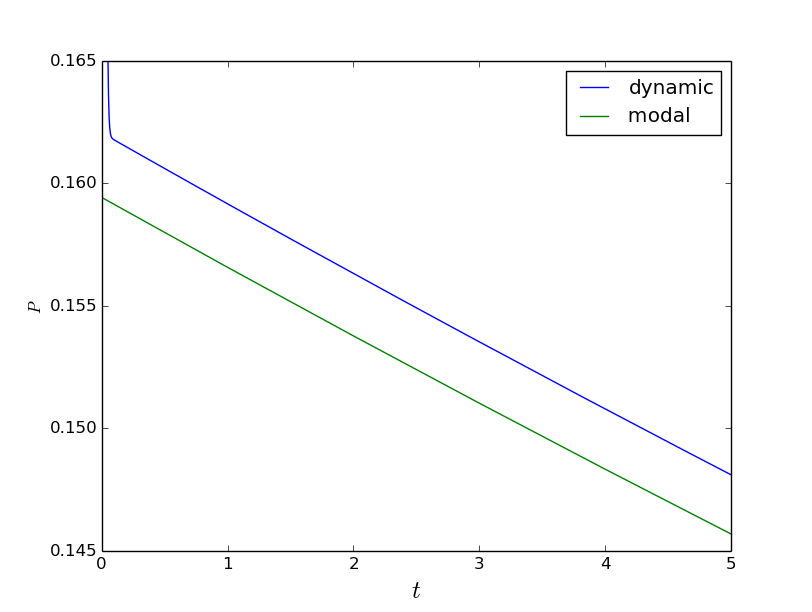
\includegraphics[width=1\linewidth] {17.png}
\begin{center}
Fig 5. Neutronic power
\end{center}
\end{minipage}
\begin{minipage}{0.5\textwidth}
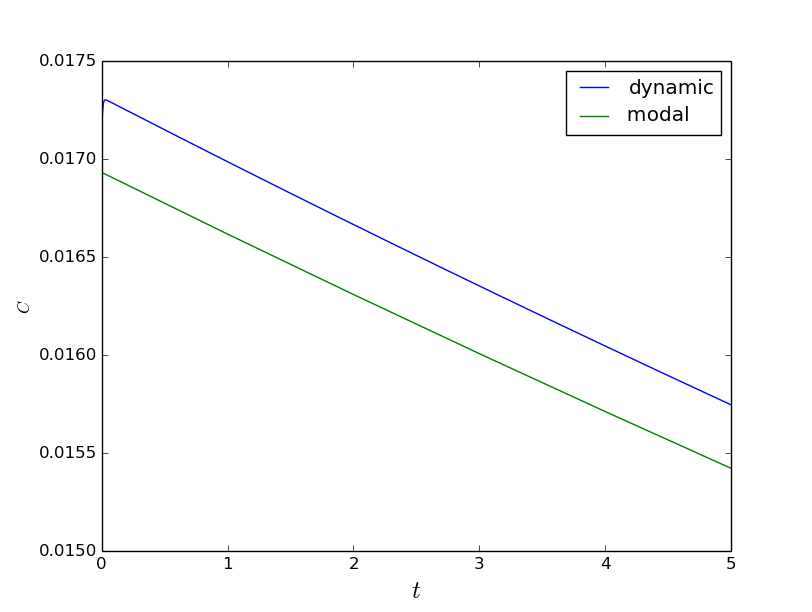
\includegraphics[width=1\linewidth] {18.png}
\begin{center}
Fig 6. Delayed neutrons sourse
\end{center}
\end{minipage}

\vspace{0.5em}
The dynamics of the slow phase is illustrated in Figs. 5, 6.
}


\end{poster}

\end{document}